%% The first command in your LaTeX source must be the \documentclass comand. This is the generic manuscript mode required for submission and peer review.
%\documentclass[sigconf]{acmart} % two column
\documentclass[manuscript,authorversion,nonacm]{acmart} % one column

%\documentclass[sigconf,authorversion,nonacm]{acmart}

%% To ensure 100% compatibility, please check the white list of
%% approved LaTeX packages to be used with the Master Article Template at
%% https://www.acm.org/publications/taps/whitelist-of-latex-packages

% Packages here:
\usepackage{subcaption}
\usepackage{multirow}
\usepackage{colortbl}
\usepackage[table,xcdraw]{xcolor}
\usepackage[table]{xcolor}
\usepackage{balance}
\usepackage{soul}
\usepackage{graphicx}
\usepackage{enumitem}
\usepackage{wrapfig}
\usepackage{makecell}

% Beamer presentation requires \usepackage{colortbl} instead of \usepackage[table,xcdraw]{xcolor}
% \usepackage[normalem]{ulem}
% \useunder{\uline}{\ul}{}

% remove author addresses at bottom of title page
\makeatletter
\let\@authorsaddresses\@empty
\makeatother

% for block quotes
\usepackage{etoolbox}
% \AtBeginEnvironment{quote}{\par\singlespacing\small}

%%
%% \BibTeX command to typeset BibTeX logo in the docs
\AtBeginDocument{%
  \providecommand\BibTeX{{%
    \normalfont B\kern-0.5em{\scshape i\kern-0.25em b}\kern-0.8em\TeX}}}

\settopmatter{printacmref=false}

%%
%% end of the preamble, start of the body of the document source.

\begin{document}

%%
%% The ``title`` command has an optional parameter,
%% allowing the author to define a ``short title`` to be used in page headers.
\title[Preliminary Report: Your project title here]{Preliminary Report: Your project title here}

%%
%% The ``author`` command and its associated commands are used to define
%% the authors and their affiliations.

\author{Put your group names here (first and last)}
\affiliation{%
  \institution{CMPU 250}
  \city{Spring 2025}
  \country{Vassar College}
}

%% short names on header of each page
\renewcommand{\shortauthors}{Short author names (just last names)}

\maketitle

%%%%%%%%%%%%%%%%%%%%%%%%%%%%%%%%%%%%%%%%%%%%%


\section{Introduction}

This is an introduction to your report.

Fill in rest of report here (with appropriate sections)


\begin{figure}[h]
    \centering
    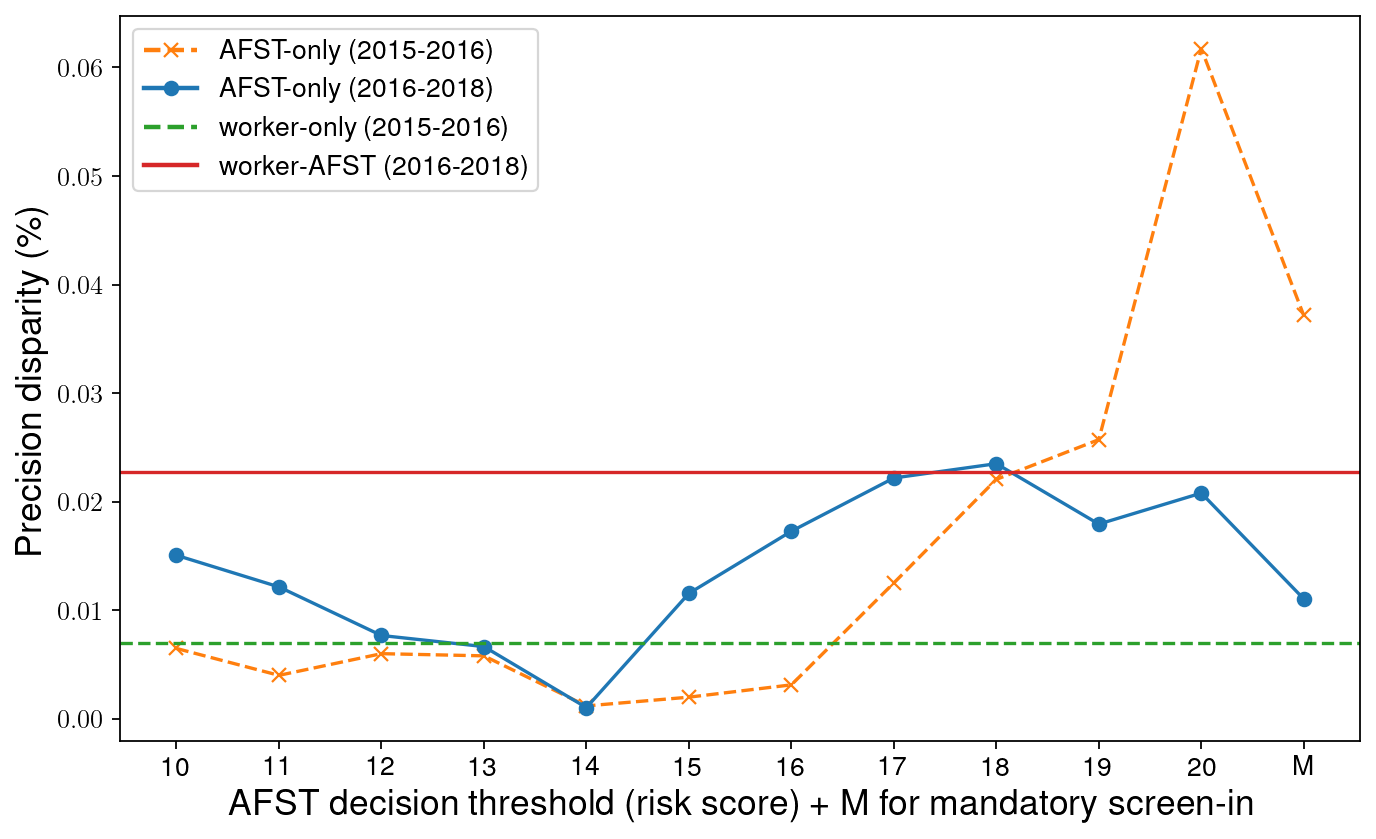
\includegraphics[width = 0.7 \linewidth]{Source/figures/precision_disparity.png} 
    \caption{This is an example figure.} 
    \label{fig:precision-disparity}
    \Description[This is an alt text --- a description of the image in the figure for making your paper accessible. See here for best practices: https://accessibility.huit.harvard.edu/describe-content-images]{This is an alt text --- a description of the image in the figure for making your paper accessible. See here for best practices: https://accessibility.huit.harvard.edu/describe-content-images}
\end{figure}


% bibliography
\newpage
\bibliographystyle{ACM-Reference-Format}
\bibliography{reference}


% appendix (if necessary)
\newpage 
\appendix


\end{document}